% Layered Bitemporal Graphs — open-access preprint draft.
% Build: see paper/README.md (pdflatex + bibtex, TeX Live basic is enough).
\documentclass[11pt]{article}

\usepackage[T1]{fontenc}
\usepackage[utf8]{inputenc}
\usepackage{lmodern}
\usepackage[a4paper,margin=1in]{geometry}
\usepackage{amsmath,amssymb,amsthm,mathtools}
\usepackage{microtype}
\usepackage{booktabs,array}
\newcolumntype{L}[1]{>{\raggedright\arraybackslash}p{#1}}
\usepackage{xcolor}
\usepackage{url}
\usepackage[numbers,sort&compress]{natbib}
\usepackage{caption}
\usepackage{tikz}
\usetikzlibrary{arrows.meta,positioning,fit,backgrounds,calc,shapes.geometric}
\usepackage[colorlinks=true,linkcolor=blue!50!black,citecolor=green!40!black,urlcolor=blue!50!black]{hyperref}

% ---------------------------------------------------------------- theorems
\theoremstyle{plain}
\newtheorem{theorem}{Theorem}
\newtheorem{lemma}[theorem]{Lemma}
\newtheorem{proposition}[theorem]{Proposition}
\newtheorem{corollary}[theorem]{Corollary}
\theoremstyle{definition}
\newtheorem{definition}{Definition}
\newtheorem{example}{Example}
\theoremstyle{remark}
\newtheorem{remark}{Remark}

% ---------------------------------------------------------------- notation
\newcommand{\Stmt}{\mathcal{E}}          % statement identifiers
\newcommand{\Node}{\mathcal{N}}          % nodes
\newcommand{\Lit}{\mathcal{L}}           % literals
\newcommand{\Pred}{\mathcal{P}}          % predicates
\newcommand{\TT}{\mathbb{T}}             % transaction numbers
\newcommand{\VT}{\mathbb{V}}             % valid-time instants
\newcommand{\refs}{\rightarrow}          % reference relation
\newcommand{\supp}{{\downarrow}}          % support (ground) of a statement
\newcommand{\dep}{{\uparrow}}            % dependents
\newcommand{\core}{\gamma}               % ground core
\newcommand{\life}{\lambda}              % transaction-time lifetime
\newcommand{\valid}{\nu}                 % valid-time interval
\newcommand{\tadd}{t_{\mathrm{add}}}
\newcommand{\tret}{t_{\mathrm{ret}}}
\newcommand{\View}[2]{V_{#1}^{#2}}
\newcommand{\enc}{\mathsf{enc}}
\newcommand{\dec}{\mathsf{dec}}
\newcommand{\sys}[1]{\texttt{sys:#1}}
\newcommand{\mg}[1]{\texttt{mg:#1}}
\newcommand{\iri}[1]{\texttt{#1}}
\newcommand{\eff}{\valid^{\ast}}
\newcommand{\Lin}{\Lambda}               % lineage predicates

\title{Layered Bitemporal Graphs:\\
Statement Identity, Two Clocks, and Metagraphs as Tags}
\author{Volodymyr Pavlyshyn\\[2pt]
\small Independent researcher\\
\small Revision 4, 3 October 2026\\
\small \href{https://github.com/Volland}{github.com/Volland}}
\date{}

\newcommand{\doi}[1]{\href{https://doi.org/#1}{\nolinkurl{#1}}}
\hypersetup{pdftitle={Layered Bitemporal Graphs},pdfauthor={Volodymyr Pavlyshyn},pdfsubject={Revision 4: reference integrity and temporal correction}}
\begin{document}
\maketitle

% =====================================================================
\begin{abstract}
Agent memory needs durable statement identity, provenance, and a distinction
between when a claim held and when the system recorded it. We study layered
bitemporal graphs, in which statement occurrences can reference other
occurrences and carry both transaction-time lifetimes and valid-time intervals.
On a referentially complete history, reference-closed sets form an Alexandrov
topology. Its interior operator, the ground core, characterises minimal
retraction cascades, grounded snapshots, and effective valid-time intervals.
We give a correction contract that preserves structural closure under explicit
patch and lineage conditions; preservation of references excludes changes made
to the corrected root. A typed anchor-and-role encoding of metagraphs commutes
with well-formed bitemporal snapshots. Compact binary encodings require additional
acyclicity for insertion under a live-reference discipline. The calculus is
realised in Tiramemsu, an embedded SQLite graph database. Retained checks
identified four implementation gaps; endpoint validation, closed retention and
transaction-date guards now prevent those counterexamples. These checks support
selected contracts rather than certifying the entire implementation. Our contribution is an operational account of recursive temporal
reference integrity, rather than a new theory of temporal databases or finite
topologies.

\end{abstract}

% =====================================================================
\section{Introduction}\label{sec:intro}

Consider an agent that reads in a chat log that Alice works at Acme. It records
the fact, notes that it is 80\% confident, that the source was a particular
conversation, and that a belief it holds elsewhere is supported by this fact.
A month later, Alice says she actually joined in February, not January. A week
after that, an auditor asks what the agent believed on the 3rd of March, on
what evidence, and since when.

Each part of this scenario has a mature answer in some literature. Annotating
a fact needs statement-level identity, as in reification, RDF-star and RDF~1.2
\cite{hartig2017rdfstar,w3c2026rdf12concepts}, singleton properties
\cite{nguyen2014singleton}, Wikidata qualifiers \cite{hernandez2015reifying},
the Amazon Neptune OneGraph model \cite{lassila2023onegraph} and the domain graph
of MillenniumDB \cite{vrgoc2023millenniumdb}. Distinguishing \emph{when it was
true} from \emph{when we knew} is the bitemporal model of temporal databases
\cite{snodgrass1985taxonomy,jensen1994unifying,jensen1998glossary,snodgrass1999developing},
standardised in SQL:2011 \cite{kulkarni2012temporal}. Historical versions are queryable under normal operations in Datomic
\cite{datomic} and XTDB \cite{xtdb}; explicit history-removal operations,
such as XTDB's ERASE, fall outside our never-forget discipline. Withdrawing everything that rests on a withdrawn premise is the
job of truth maintenance systems \cite{doyle1979tms,dekleer1986atms}.
Grouping facts into larger units that can themselves be related is the
metagraph \cite{basu2007metagraphs,chernenkiy2017rdf,gapanyuk2021development,goertzel2020folding}.

What is less studied is what happens when all of these live in \emph{one}
structure, at the granularity of a single statement. Then annotations have
lifetimes, corrections must carry annotations along, a valid-time slice can
contain a confidence score whose fact is not valid at that instant, and a
container can be retracted while its contents stay. This paper gives that
combined structure a precise semantics and proves the properties that make it
safe to build on.

\paragraph{Contributions.}
\begin{enumerate}
\item A formal model of \emph{layered bitemporal graphs} (LBGs): statements with
  identity, a reference relation between statements, transaction-time lifetimes
  and valid-time intervals (Sections~\ref{sec:model} and~\ref{sec:time}).
\item An application of the standard down-set construction \cite{barmak2011finite}:
  the \emph{ground core} $\core$ identifies grounded sets with the open sets
  of an Alexandrov topology
  (Lemma~\ref{lem:core}).
\item Theorems on the operations: stability of time travel
  (Theorem~\ref{thm:stability}), minimality of the retraction cascade
  (Theorem~\ref{thm:cascade}), groundedness of snapshots as lifetime nesting
  (Theorem~\ref{thm:nesting}), effective validity (Theorem~\ref{thm:effective}),
  and correctness of correction by cascade-and-replay
  (Theorem~\ref{thm:supersede}) (Section~\ref{sec:ops}).
\item A faithful encoding of temporal metagraphs into LBGs and the
  \emph{Bitemporal Lifting Theorem} (Theorem~\ref{thm:lifting}), with corollaries
  for unfold, nesting, fold and container retraction (Section~\ref{sec:metagraph}).
\item A realisation in an embedded database and a conformance analysis: four conformance repairs, with retained regression checks and explicit evidence
  limits
  (Section~\ref{sec:impl}).
\end{enumerate}

\paragraph{Terminology.} \emph{Layered} here means stratified by reference:
a statement about a statement sits one layer above it. This is not the
\emph{multilayer network} of network science \cite{kivela2014multilayer},
where layers are parallel edge sets over a shared vertex set. It is close to the
\emph{multilayer graphs} of Angles et al.\ \cite{angles2022multilayer}, in which
edges have identifiers and can be endpoints of other edges; we add the two clocks
and the operations that keep such structures consistent over time.

% =====================================================================
\section{Background and Related Work}\label{sec:related}

\paragraph{Bitemporal data.}
Snodgrass and Ahn separated \emph{valid time}, when a fact holds in the
modelled world, from \emph{transaction time}, when it is current in the
database \cite{snodgrass1985taxonomy}. The Bitemporal Conceptual Data Model
attaches to each tuple a set of bitemporal chronons and shows that several
representational models are snapshot-equivalent views of it
\cite{jensen1994unifying}. The consensus glossary fixes the vocabulary
\cite{jensen1998glossary}, and SQL:2011 introduced application-time and
system-versioned tables \cite{kulkarni2012temporal}. Our lifetimes and valid intervals follow these two time dimensions.
Temporal referential integrity already occurs in flat relations: a child
period must be covered by matching parent periods \cite[Section 2.2.2]{kulkarni2012temporal}.
Here references are to individual immutable occurrences, and may nest recursively.
We specialise that established integrity problem to occurrence references,
structural cascades, and correction by replay.

\paragraph{Temporal graphs.}
Network science studies graphs whose edges are active at times, and
time-respecting paths along them
\cite{kempe2002connectivity,holme2012temporal,casteigts2012tvg}. Wu et al.\
give efficient algorithms for earliest-arrival, latest-departure, fastest and
shortest temporal paths \cite{wu2014path}. In databases, temporal
property-graph models attach intervals to nodes and edges
\cite{debrouvier2021tgraph,rost2022gradoop} and temporal RDF attaches them to
triples \cite{gutierrez2007time}. These cited models motivate temporal graph queries. Our comparison concerns
their published representations, rather than an impossibility claim about
encodings: ordinary reification can represent higher-order dependencies. We
make those dependencies explicit at the level of temporal statement occurrences
and study their closure under correction.
Systems work on temporal graph stores, such as AeonG \cite{hou2024aeong},
Clock-G \cite{massri2022clockg} and ChronoGraph \cite{byun2020chronograph},
optimises the storage and traversal of versioned vertices and edges, and temporal
graph algebra \cite{moffitt2017tga} gives point- and interval-based semantics
for evolving graphs.

\paragraph{Statement-level identity.}
RDF reification, RDF-star \cite{hartig2017rdfstar} and the RDF~1.2 reifier
model \cite{w3c2026rdf12concepts} let a triple be talked about.
A quoted triple identifies content, not by itself an occurrence; RDF~1.2 reifiers
are resources that relate to triple terms. The cited RDF~1.2 document is a
Candidate Recommendation Snapshot, not a final Recommendation. Singleton
properties mint a predicate per occurrence \cite{nguyen2014singleton}.
Hern\'andez, Hogan and Kr\"otzsch compared these encodings for Wikidata's
qualified statements \cite{vrandecic2014wikidata,hernandez2015reifying}, and
benchmarks show the cost of encoding statement metadata on top of plain triples
\cite{frey2019metadata,orlandi2021benchmarking}. Named graphs group triples
under a name that can carry provenance \cite{carroll2005named}. OneGraph
\cite{lassila2023onegraph} and MillenniumDB's domain graph
\cite{vrgoc2023millenniumdb} make every edge an object with an identifier. Gelling, Fletcher and Schmidt's
\emph{statement graphs} \cite{gelling2024statement} make statement identity the
unifying primitive of RDF, RDF-star and property graphs, and are the closest data
model to ours; Angles et al.'s multilayer graphs \cite{angles2022multilayer} are
another. Their cited presentations emphasise graph-model interoperability;
we study an additional temporal correction contract rather than claiming that
those representations cannot encode time or containment. In our model, each \emph{occurrence} of a
statement has an identifier, properties included. Unlike RDF~1.2, where a
reifier may stand for several triples and a triple for several reifiers, our
identifier is a total function to content.

\paragraph{Metagraphs and hypergraphs.}
Basu and Blanning define a metagraph over a generating set with edges between
\emph{sets} of elements \cite{basu2007metagraphs}. Chernenkiy, Gapanyuk and
colleagues add metavertices and metaedges that contain fragments, and
annotations that are themselves metagraphs \cite{chernenkiy2017rdf,gapanyuk2021development}.
Goertzel develops morphism-based folding and unfolding \cite{goertzel2020folding};
our membership-tag operation below is a narrower storage operation, not a
claim to implement that entire algebra. HypergraphDB stores hyperedges that can point
to hyperedges \cite{iordanov2010hypergraphdb}. The use of metagraphs for agent
memory is discussed in the author's self-published book \cite{pavlyshyn2026metagraph}.
Definition~\ref{def:metagraph} combines set-valued endpoints, higher-order atoms
and membership occurrences; it is not an identification of these traditions.
We establish snapshot lifting for this explicit variant under temporal
well-formedness (Theorem~\ref{thm:lifting}).

\paragraph{Truth maintenance and belief revision.}
A justification-based TMS withdraws every belief whose justification loses
support \cite{doyle1979tms}; an assumption-based TMS tracks the assumption sets
under which beliefs hold \cite{dekleer1986atms}. AGM belief revision axiomatises
contraction and revision of theories \cite{alchourron1985logic}. Our cascade is a
syntactic, monotone cousin of TMS withdrawal. Support is structural (a layer
rests on its base), there are no alternative justifications, and nothing is
forgotten, because withdrawal closes a lifetime. Theorem~\ref{thm:cascade}
plays the role of a minimal-change postulate: the cascade withdraws exactly what
it must and nothing more.

\paragraph{Provenance.}
Why- and where-provenance \cite{buneman2001why} and provenance semirings
\cite{green2007provenance} annotate query answers with the source tuples that
produced them. Statement identity makes such citations durable, because a cited
statement can later be checked for retraction in any snapshot.

\paragraph{Agent memory.}
Recent agent-memory systems store temporal knowledge graphs whose edges carry
validity windows and system times; Zep's Graphiti is a prominent example
\cite{rasmussen2025zep}. Other memory layers manage what enters a bounded context
\cite{packer2023memgpt}, extract and consolidate memories
\cite{chhikara2025mem0,xu2025amem}, or retrieve over a knowledge graph
\cite{gutierrez2024hipporag}; benchmarks such as LongMemEval test knowledge updates
and temporal reasoning explicitly \cite{wu2024longmemeval}. Our analysis
complements these cited agent-memory architectures with an explicit contract
for structural annotation replay; we do not claim an exhaustive comparison
against every system version. The surveys of knowledge graphs \cite{hogan2021knowledge}
summarise the broader design space. Our model can be read as giving such
systems a precise account of what a correction, a retraction or a snapshot
does to the annotations on a fact.

% =====================================================================
\begin{table}[t]
\centering\small
\begin{tabular}{L{3.0cm}L{4.2cm}L{6.3cm}}
\toprule Cited representation & Established mechanism & Relation to this paper \\
\midrule
SQL:2011 \cite{kulkarni2012temporal} & Temporal periods and referential constraints & Predecessor for temporal coverage; our targets are immutable occurrences with recursive dependencies. \\
Statement graphs \cite{gelling2024statement} & Identity and cross-model mappings & Closest structural model; we add a scoped temporal operation contract. \\
Multilayer graphs \cite{angles2022multilayer} & Identified edges as endpoints & Shared higher-order primitive; we analyse reference closure across two clocks. \\
Graphiti/Zep preprint \cite{rasmussen2025zep} & Temporal agent-memory architecture & Application context; no completeness or impossibility claim about later versions. \\
\bottomrule
\end{tabular}
\caption{Comparison against the cited publications, not all possible encodings or later releases.}
\end{table}

\section{Layered Graphs}\label{sec:model}

\begin{table}[t]
\centering\small
\begin{tabular}{ll}
\toprule Symbol & Meaning \\
\midrule
$S,\kappa$ & Complete occurrence history and immutable triple content \\
$X,V_t,V^v$ & A row set, as-of view, and valid-at slice \\
$\refs,\refs_{\Lin}$ & Full references and references excluding lineage predicates \\
$\core,\core_{\Lin}$ & Full and structural ground cores \\
$\dep_X r$ & Full reference dependents inside the induced live graph \\
$\life,\valid$ & Transaction lifetime and claimed valid interval \\
$C,F,R,\sigma$ & Cascade, dropped memberships, retained set, fresh-copy map \\
\bottomrule
\end{tabular}
\caption{Notation. Lineage still requires allocated historical targets.}
\end{table}

\subsection{Statements and references}

Fix disjoint countable sets: nodes $\Node$, literals $\Lit$, statement
identifiers $\Stmt$ and transaction numbers $\TT=\{1,2,\dots\}$. Predicates are
nodes, $\Pred\subseteq\Node$.

\begin{definition}[Layered graph]\label{def:lg}
A \emph{layered graph} is a finite set $S\subseteq\Stmt$ of statements together
with a content function $\kappa\colon S\to(\Node\cup\Stmt\cup\TT)\times\Pred\times(\Node\cup\Lit\cup\Stmt\cup\TT)$,
written $\kappa(e)=(s_e,p_e,o_e)$, such that no statement mentions itself:
$s_e\neq e\neq o_e$, and every statement-valued subject or object belongs
to $S$. Thus the history is \emph{referentially complete}; its views need not be.
\end{definition}

The identifier $e$ is the identity of one \emph{occurrence} of a fact. Two
statements may have equal content (parallel edges); content is immutable. A
statement whose object is a literal is a property; one whose subject or object
is a statement is a layer or a citation.

\begin{definition}[References, support, dependents]
For $e,e'\in S$ write $e\refs e'$ if $e'\in\{s_e,o_e\}$. Let $\refs^{*}$ be the
reflexive--transitive closure. The \emph{support} of $e$ is
$\supp e=\{e'\in S : e\refs^{*}e'\}$, everything $e$ rests on, $e$ included. For
$X\subseteq S$ the \emph{dependents} of $e$ in $X$ are
$\dep_X e=\{x\in X : x\refs_X^{*}e\}$, where $\refs_X$ is the
reference relation induced on $X$. On a grounded $X$, this equals reachability
in the whole history restricted to starting points in $X$.
\end{definition}

The relation $\refs$ may contain cycles of length at least two (statement $a$
about $b$ about $a$). Proposition~\ref{prop:acyclic} shows that cycles cannot
arise under the live-reference discipline of Section~\ref{sec:ops}. Where
$\refs$ is acyclic the \emph{rank} of a statement, $0$ if it references no
statement and otherwise one more than the largest rank it references, is the
layer it sits in.

\begin{figure}[t]
\centering
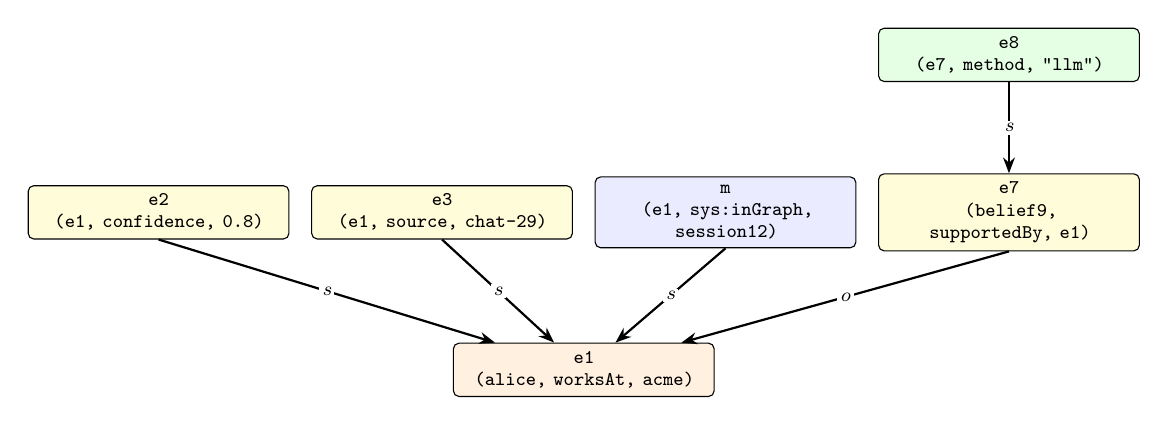
\begin{tikzpicture}[
  st/.style={draw,rounded corners=2pt,fill=#1,inner sep=3pt,font=\scriptsize\ttfamily,align=center,text width=3.1cm},
  st/.default=white,
  ref/.style={-{Stealth[length=2mm]},thick},
  lab/.style={font=\scriptsize\itshape,fill=white,inner sep=1pt}]
\node[st=orange!12] (e1) at (0,0) {e1\\(alice, worksAt, acme)};
\node[st=yellow!15] (e2) at (-5.4,2) {e2\\(e1, confidence, 0.8)};
\node[st=yellow!15] (e3) at (-1.8,2) {e3\\(e1, source, chat-29)};
\node[st=blue!8]    (m)  at (1.8,2)  {m\\(e1, sys:inGraph, session12)};
\node[st=yellow!15] (e7) at (5.4,2)  {e7\\(belief9, supportedBy, e1)};
\node[st=green!10]  (e8) at (5.4,4)  {e8\\(e7, method, "llm")};
\draw[ref] (e2.south) -- node[lab]{s} (e1);
\draw[ref] (e3.south) -- node[lab]{s} (e1);
\draw[ref] (m.south) -- node[lab]{s} (e1);
\draw[ref] (e7.south) -- node[lab]{o} (e1);
\draw[ref] (e8) -- node[lab]{s} (e7);
\end{tikzpicture}
\caption{A layered graph. Rows are ranks 0, 1 and 2. Arrows are the reference
relation $\refs$, labelled by the position (subject or object) that holds the
referenced statement. The
support of \texttt{e8} is $\{\texttt{e8},\texttt{e7},\texttt{e1}\}$; the
dependents of \texttt{e1} are all six statements. The membership \texttt{m}
places \texttt{e1} in a named graph, and is itself a statement.}
\label{fig:layers}
\end{figure}

\subsection{Grounded sets and the ground core}

The central notion instantiates the established correspondence between finite
preorders and Alexandrov spaces \cite{barmak2011finite}. We claim the operational
application below, not the topology construction itself.

\begin{definition}[Grounded set, ground core]
A set $X\subseteq S$ is \emph{grounded} if $\supp e\subseteq X$ for every
$e\in X$, that is, if $e\in X$ and $e\refs e'$ imply $e'\in X$. The
\emph{ground core} of an arbitrary $X\subseteq S$ is
\[\core(X)=\{e\in X : \supp e\subseteq X\}.\]
\end{definition}

A grounded set never contains an annotation without the statement it
annotates, nor a citation without what it cites. A raw engine state with an
unallocated endpoint is outside Definition~\ref{def:lg}. For such a state,
let $B$ be the rows with a missing statement-valued endpoint. Remove $B$ and
all its reverse-reachable dependents before applying $\core$ to the remaining,
referentially complete carrier. This separate integrity check prevents missing
identifiers from disappearing from the formal reference relation.

\begin{lemma}[Ground core]\label{lem:core}
For all $X,Y\subseteq S$ and families $(X_i)_{i\in I}$:
\begin{enumerate}
\item $\core(X)\subseteq X$, $\core(\core(X))=\core(X)$, and $X\subseteq Y$ implies $\core(X)\subseteq\core(Y)$;
\item $\core(X)$ is grounded, and it is the largest grounded subset of $X$;
\item $\core\bigl(\bigcap_i X_i\bigr)=\bigcap_i\core(X_i)$;
\item arbitrary unions and intersections of grounded sets are grounded.
\end{enumerate}
Hence the grounded sets are the open sets of an Alexandrov topology on $S$, and
$\core$ is its interior operator.
\end{lemma}

\begin{proof}
(1) Deflation and monotonicity are immediate. If $e\in\core(X)$ and
$e'\in\supp e$ then $\supp e'\subseteq\supp e\subseteq X$ by transitivity, so
$\supp e\subseteq\core(X)$; this shows $e\in\core(\core(X))$ and also that
$\core(X)$ is grounded. (2) If $Y\subseteq X$ is grounded and $e\in Y$, then
$\supp e\subseteq Y\subseteq X$, so $e\in\core(X)$. (3) $\supp e\subseteq\bigcap_i X_i$
iff $\supp e\subseteq X_i$ for all $i$. (4) The defining condition is preserved
by arbitrary unions and intersections. A topology closed under arbitrary
intersections is Alexandrov; its open sets here are the down-sets of the
preorder $\refs^{*}$.
\end{proof}

\begin{lemma}[Cascade as a core]\label{lem:cascade-core}
If $X$ is grounded and $e\in X$, then $X\setminus\dep_X e=\core(X\setminus\{e\})$.
\end{lemma}

\begin{proof}
Let $x\in X\setminus\{e\}$. Because $X$ is grounded, $\supp x\subseteq X$, so
$\supp x\subseteq X\setminus\{e\}$ iff $e\notin\supp x$ iff $x\notin\dep_X e$. The
statement $e$ itself lies in $\dep_X e$ and not in $X\setminus\{e\}$.
\end{proof}

% =====================================================================
\section{Two Clocks}\label{sec:time}

\subsection{Lifetimes and intervals}

Transaction numbers are gap-free and strictly increasing, one per committed
transaction. Valid-time instants $\VT$ form a total order (epoch milliseconds in
the implementation); $\pm\infty$ denote unbounded ends. All intervals are
half-open.

\begin{definition}[Layered bitemporal graph]
A \emph{layered bitemporal graph} (LBG) is a layered graph $(S,\kappa)$ with two
further functions on $S$: a \emph{lifetime}
$\life(e)=[\tadd(e),\tret(e))$ with $\tadd(e)\in\TT$ and
$\tret(e)\in\TT\cup\{\infty\}$, $\tadd(e)\le\tret(e)$; and a \emph{valid
interval} $\valid(e)=[v_{\mathrm{from}}(e),v_{\mathrm{to}}(e))\subseteq\VT$,
non-empty. Content $(\kappa(e),\valid(e))$ is immutable; only
$\tret(e)$ may change, once, from $\infty$ to a transaction number.
\end{definition}

A statement with $\tadd(e)=\tret(e)$ was asserted and retracted inside one
transaction and is visible in no snapshot. Changing a valid interval is a
correction (Section~\ref{sec:supersede}), never an update.

\begin{definition}[Views]
For $t\in\TT$ and $v\in\VT$:
\[
V_t=\{e\in S: t\in\life(e)\},\qquad
V^{v}=\{e\in S: v\in\valid(e)\},\qquad
\View{t}{v}=V_t\cap V^{v}.
\]
$V_t$ is the \emph{as-of} view, $V^{v}$ the \emph{valid-at} slice, and
$\View{t}{v}$ the bitemporal snapshot. The \emph{history} view is $S$ itself.
\end{definition}

A query evaluated on a view sees the content of exactly the statements in the
view. The implementation lets each pattern of a query choose its own view;
here one view per query is enough.

\subsection{Histories and stability}

A database evolves by committed transactions. Let $S^{(t)}$ denote the LBG
after transaction $t$, with $\tret=\infty$ for statements still live. A
transaction $t$ may only (a) insert statements with $\tadd=t$ and fresh
identifiers, and (b) set $\tret(e)=t$ for statements live at that operation,
including ones inserted earlier within $t$. Content remains immutable.
This is the \emph{never-forget} discipline: no row is deleted and no identifier
is reused. The engine supplies the transaction protocol. Database triggers
prevent deletion, replacement and content changes. Format 3 also validates
current-transaction dates against the committed watermark, assuming the schema
and engine metadata remain intact (Section~\ref{sec:impl}).

\begin{theorem}[Stability of time travel]\label{thm:stability}
For all $t\le t'\le t''$, the view $V_t$ computed in $S^{(t')}$ equals $V_t$
computed in $S^{(t'')}$, statement for statement and with equal content.
Moreover, $V_t$ equals the set obtained by replaying, in order, the insert and
retract events with transaction number at most $t$, processing each occurrence's
addition before its retraction when their transaction numbers agree.
\end{theorem}

\begin{proof}
Every transaction $u\in(t',t'']$ inserts statements with $\tadd=u>t$, which
are not in $V_t$, and sets $\tret(e)=u>t$ on statements that were live, which
keeps $t\in\life(e)$ exactly when it held before. Content never changes. For
the second claim, a statement is in the replayed set iff its insert event has
time $\le t$ and its retract event, if any, has time $>t$, which is the
definition of $V_t$.
\end{proof}

The theorem is what makes an answer \emph{about the past} reproducible: a
snapshot never changes once its transaction has committed. The second half is
checked in the implementation by property-based tests over random operation
sequences.

% =====================================================================
\section{Operations and Their Guarantees}\label{sec:ops}

\subsection{Assert and create}

\emph{Assert}$(s,p,o,\valid)$ returns an existing live occurrence with the
same triple and an overlapping valid interval, or inserts a fresh one.
The implementation chooses the smallest matching eid. Returning an existing
occurrence does not extend its interval to cover the requested interval; callers
that need a distinct episode use create or an explicit correction. Here
``same triple'' excludes the valid interval, which is also immutable content. \emph{Create} always inserts, which is
how parallel edges are made. Both insert statements whose subject or object may
be another statement. What they are allowed to reference decides whether
snapshots stay grounded.

\begin{definition}[Live-reference discipline]
Let $\Lin\subseteq\Pred$ be a set of \emph{lineage} predicates. A transaction
satisfies the \emph{live-reference discipline} (LR) if every statement $e$ it
inserts with $p_e\notin\Lin$ references only statements that are live at the
moment of insertion (inserted earlier and not retracted).
\end{definition}

Write $\refs_{\Lin}$ for the restriction of $\refs$ to statements whose
predicate is not in $\Lin$, and call a set \emph{structurally grounded} when it is
grounded for $\refs_{\Lin}$. Write $\supp_{\Lin}$, $\dep_{\Lin,X}$ and
$\core_{\Lin}$ for support, induced dependents and the core computed with this
relation. All results about $\core$ apply to this relation as well. Full
reference closure and structural closure are different: lineage links may point
to historical occurrences outside the live view, but never to missing identifiers.
LR imposes liveness only on non-lineage references; all endpoints must already
exist except during an explicitly specified atomic replay.

\subsection{Retraction and its cascade}

Retracting $e$ retracts, in the same transaction, $e$ and every live statement
that transitively references it through a subject or object position: its
layers, the statements that cite it, the layers on those, and so on. Nodes
never cascade.

\begin{theorem}[Cascade minimality]\label{thm:cascade}
Let $X$ be the live set before a retraction of $e\in X$, and let $X$ be
grounded. The cascade retracts exactly $\dep_X e$, and:
\begin{enumerate}
\item $X\setminus\dep_X e=\core(X\setminus\{e\})$, so the remaining live set is grounded;
\item $\dep_X e$ is the \emph{least} set $R$ such that $e\in R\subseteq X$ and $X\setminus R$ is grounded.
\end{enumerate}
\end{theorem}

\begin{proof}
The cascade is a breadth-first search from $e$ over inverse references among
live statements, with a visited set, so it terminates on cycles and reaches
exactly $\dep_X e$. Claim~1 is Lemma~\ref{lem:cascade-core}. For Claim~2, let
$R$ be any such set. Then $X\setminus R$ is a grounded subset of
$X\setminus\{e\}$, hence contained in its core $X\setminus\dep_X e$ by
Lemma~\ref{lem:core}(2), so $\dep_X e\subseteq R$.
\end{proof}

For structural closure the theorem applies to $\refs_{\Lin}$: its minimal
retraction is $\dep_{\Lin,X}e$. The engine follows all live references, including
lineage, and may retract more than this structural minimum. The full-reference
minimality claim therefore requires full groundedness.

Under its stated hypothesis, the theorem says that the cascade is forced. Any retraction that leaves memory
grounded must take at least $\dep_X e$ with it, and the cascade takes nothing
else. In belief-revision terms it is the minimal contraction for the
structural support relation. The same set can be computed without the writer,
as a read on any view: as-of $t$ it shows what depended on $e$ then. It is also
the set of ends of the regular path $(\hat{}\,\sys{subject}\mid\hat{}\,\sys{object})^{*}$
from $e$. Both equivalences are checked by property tests in the
implementation.

\subsection{Snapshots are grounded exactly when lifetimes nest}

\begin{theorem}[Transaction-time nesting]\label{thm:nesting}
For a history $S$ the following are equivalent:
\begin{enumerate}
\item every as-of view $V_t$ is structurally grounded;
\item for every structural reference $e\refs_{\Lin}e'$, $\life(e)\subseteq\life(e')$.
\end{enumerate}
Starting from the empty history, if insertions satisfy LR, retractions follow
all live references, and corrections satisfy Theorem~\ref{thm:supersede},
then both hold.
\end{theorem}

\begin{proof}
(1)$\Leftrightarrow$(2): $V_t$ is grounded for every $t$ iff for each reference
$e\refs_{\Lin}e'$ and each $t$, $t\in\life(e)$ implies $t\in\life(e')$, which
is $\life(e)\subseteq\life(e')$. For the sufficient condition we show by
induction over the operations of each transaction that the live set stays
structurally grounded; the committed live set after $t$ is $V_t$, because a
statement inserted and retracted within $t$ has an empty lifetime. Insertion
under LR adds a statement whose structural referents are live. Retraction
preserves groundedness by Theorem~\ref{thm:cascade}, applied to
$\refs_{\Lin}$-dependents (the implementation's cascade follows all references,
lineage included; the remaining set is still structurally grounded, because if
$x\refs_{\Lin}y$ and $y$ is removed then $x\refs y\refs^{*}e$, so $x$ is removed
too). Correction is covered by
Theorem~\ref{thm:supersede}.
\end{proof}

Condition~2 gives a geometric reading of a grounded history. Draw each
lifetime as a segment on the transaction axis; a layer's segment lies inside
the segment of the statement it rests on. Lineage links are the opposite case:
their segment begins exactly where the referenced statement's segment ends.

\begin{example}[Why LR is needed]\label{ex:counter}
Assert $e_1=(\iri{alice},\iri{worksAt},\iri{acme})$ at $t=1$, retract it at
$t=2$, and at $t=3$ assert $e_2=(e_1,\iri{confidence},0.8)$. Then
$e_2\in V_3$ but $e_1\notin V_3$: the as-of view at $3$ holds a confidence about
nothing. Condition~2 fails, since $\life(e_2)=[3,\infty)\not\subseteq[1,2)=\life(e_1)$.
\end{example}

\begin{proposition}[Acyclicity]\label{prop:acyclic}
Starting from the empty history, suppose ordinary and lineage insertions
reference only already-existing identifiers. Suppose correction copies preserve
an acyclic reference graph and the patched root adds no reference inside its
replay set. Then the full history is acyclic and rank is well defined. A patch
whose new statement-valued object belongs to $X\setminus C$ meets the latter
condition.
\end{proposition}

\begin{proof}
Ordinary insertion cannot close a cycle because existing immutable statements
cannot mention its fresh identifier. Replay copies an acyclic induced graph;
references leaving the copies point to old identifiers, none of which can point
back to a fresh copy. Removing or replacing a root reference by an old target
outside $C$ does not add an internal cycle. The new lineage statement is inserted
last and refers only to existing identifiers. Induction proves the claim.
\end{proof}

LR ensures existing targets for ordinary insertions, but lineage insertion must
also reject unallocated targets. An arbitrary patch into its own replay set can
create a cycle and is not covered by this proposition.

Under acyclicity, the cascade of $e$ contains only statements of strictly
higher rank than $e$ (apart from $e$): retraction propagates upward through
the layers and never sideways.

\subsection{Valid time does not nest, and how to read it}\label{sec:effective}

Valid intervals are content chosen by the writer, and a layer's interval is
independent of its base's. This is deliberate: a confidence assessed in 2026
about a fact that held in 2020 is valid in 2026. Consequently $V^{v}$, and with
it $\View{t}{v}$, need not be grounded even when every $V_t$ is. A reader who
wants a grounded slice can take its core, and the core has a closed form.

\begin{definition}[Effective validity]
For a view $X$ and $e\in X$ let
$\eff_X(e)=\bigcap\{\valid(e') : e'\in\supp e\}$ if $\supp e\subseteq X$, and
$\emptyset$ otherwise.
\end{definition}

An intersection of half-open intervals is a half-open interval, possibly empty,
so effective validity is again an interval and can be stored or indexed like any
other.

\begin{theorem}[Effective validity]\label{thm:effective}
For every view $X$ and instant $v$:
\begin{enumerate}
\item $\core(X\cap V^{v})=\{e\in X : v\in\eff_X(e)\}$, the largest grounded subset of the slice;
\item $\eff_X$ is the greatest fixpoint, under pointwise inclusion, of
$F(\varphi)(e)=\valid(e)\cap\bigcap_{e\refs e'}\varphi(e')$ on the complete
lattice $\prod_{e\in\core(X)}2^{\VT}$ ordered pointwise by inclusion.
\end{enumerate}
\end{theorem}

\begin{proof}
(1) $e\in\core(X\cap V^{v})$ iff every $e'\in\supp e$ lies in $X$ and has
$v\in\valid(e')$, iff $v\in\eff_X(e)$. Maximality is Lemma~\ref{lem:core}(2).
(2) Because $\supp e=\{e\}\cup\bigcup_{e\refs e'}\supp e'$, $\eff_X$ is a fixpoint. If
$\varphi$ is any fixpoint then $\varphi(e)\subseteq\valid(e)$ and
$\varphi(e)\subseteq\varphi(e')$ whenever $e\refs e'$, so following any reference path from $e$ to $e'$ and chaining these inclusions,
$\varphi(e)\subseteq\valid(e')$ for every $e'\in\supp e$ (cycles are harmless,
since only finite paths are used), that is
$\varphi\subseteq\eff_X$. The fixpoint also exists by Tarski's theorem
\cite{tarski1955lattice}, since $F$ is monotone on a complete lattice; the
closed form makes the theorem constructive and valid in the presence of cycles.
\end{proof}

Theorems~\ref{thm:nesting} and~\ref{thm:effective} show an asymmetry
between the clocks. Transaction time nests under the stated LR and operation contracts. Valid time is the writer's claim about the world and nests only
if the reader asks for it, through $\core$. The asymmetry is a design choice,
and the closed form reduces the reader's operation to: $\eff$ is an interval
intersection along the support, computable during the same traversal that
evaluates a layered pattern.

\subsection{Correction by cascade-and-replay}\label{sec:supersede}

Correction retracts a live root $r$ and its full live-reference cascade
$C=\dep_X r$, then replays retained occurrences under fresh identifiers.
A foreign membership is a membership in $C$ whose container is outside $C$.
Let $F$ be the foreign memberships selected for dropping. Retention must be
closed under structural references inside $C$:
\[
 R=\core_{\Lin,C}(C\setminus F),\qquad
 \core_{\Lin,C}(Y)=\{e\in Y:\supp_{\Lin,C}e\subseteq Y\},
\]
where support is computed in the structural reference graph induced on $C$.
Lineage references do not force retention and may continue to name historical
occurrences. Choose a bijection $\sigma:R\to R^{+}$ onto fresh identifiers and
extend it to a substitution $f$ that fixes all identifiers outside $R$.
In particular, dropped occurrences retain their old historical identifiers;
we do not create references to fresh identifiers for copies that were never inserted.

\begin{definition}[Admissible correction]
A correction is admissible if $X$ is structurally grounded in a referentially
complete history, $r\in R$, and the patched root has no direct self-reference
and has a non-empty valid interval. Every patched statement-valued endpoint
must exist in the extended history. If the root predicate is not lineage,
every patched statement-valued endpoint must belong to
$(X\setminus C)\cup\sigma(R)$ after substitution. Subjects and predicates are
preserved modulo $f$; the root object and valid interval may change.
The operation is atomic, adds only the replayed rows and one fresh lineage row,
and performs no other schema-induced retractions during replay.
\end{definition}

\begin{theorem}[Correction]\label{thm:supersede}
For an admissible correction at transaction $t$, replay every retained subject
and object through $f$, apply the admissible patch to the root, and insert
$\ell=(\sigma(r),\sys{supersedes},r)$ with $\sys{supersedes}\in\Lin$.
Then the new live set is
$X'=(X\setminus C)\cup\sigma(R)\cup\{\ell\}$, and:
\begin{enumerate}
\item For $x\in R\setminus\{r\}$ and $y\in R$,
  $x\refs y$ iff $\sigma(x)\refs\sigma(y)$. Non-root content and valid
  intervals are preserved modulo $f$. The root's references are preserved only
  where the patch leaves its endpoints unchanged modulo $f$.
\item $X'$ is structurally grounded and the extended history is referentially complete.
\item Every previously committed as-of view is unchanged. In particular,
  $C\cap V_{t-1}\subseteq V_{t-1}$ retains its original content permanently;
  rows inserted earlier within $t$ may belong to $C$ without belonging to $V_{t-1}$.
\end{enumerate}
For a validity-only patch all references within $R$ are preserved, so the
full induced reference structures on $R$ and $\sigma(R)$ are isomorphic.
\end{theorem}

\begin{proof}
(1) For non-root rows both endpoint positions are substituted by the injective
map $f$; old external identifiers cannot equal fresh copy identifiers. This
proves the stated equivalence. A root object patch need not preserve that relation.
(2) If a surviving old row structurally referenced a removed row, it would lie
in the full induced cascade $C$, a contradiction. For a non-root $x\in R$ and
$x\refs_{\Lin}y$, structural groundedness gives $y\in X$. If $y\in C$, closure
of $R$ gives $y\in R$, so the copy references $\sigma(y)\in X'$. Otherwise
$y\in X\setminus C$. The root meets this condition by admissibility; $\ell$ is
lineage and imposes no structural dependency. Historical lineage targets remain
allocated, and all new endpoints exist by construction or admissibility.
(3) All new rows have addition time $t$ and all retractions have time $t$.
Theorem~\ref{thm:stability} preserves every committed view with time less than $t$.
\end{proof}

\begin{remark}[Dropped memberships and schema effects]
If an implementation allocates a fresh id for every row of $C$ but inserts only
$C\setminus F$, a retained row referencing $m\in F$ can acquire a dangling target.
This violates referential completeness even for lineage; structural closure also
fails for a non-lineage reference. The specified substitution and retention rule
avoid that behavior. A membership root that is itself dropped fails $r\in R$;
its correction must be rejected or assigned an explicit alternative policy.
Cardinality or uniqueness rules that remove other rows during replay need their
own transaction contract; they are not covered by this theorem.
\end{remark}

Replay preserves structural annotations, not their truth about the replacement.
An unchanged confidence score or source citation may need revalidation after an
object patch. Applications must select a retain, drop, or revalidate policy;
this theorem describes retention of the chosen structurally closed set.
Repeated correction gives a predecessor chain in history. Replayed lineage
can also create shortcuts, and the complete chain need not exist in a live-only view.

\begin{example}[A correction timeline]
At $t=1$ create $r=(alice,worksAt,acme)$ valid on $[Jan,Jun)$, a confidence layer
$a$ valid everywhere, a container anchor $c$, and membership $m=(r,\sys{inGraph},c)$.
At $t=2$ correct only $r$'s interval to $[Feb,Jun)$ and drop $m$. Then
$C=\{r,a,m\}$, $F=\{m\}$ and $R=\{r,a\}$. The live view contains
$\sigma(r),\sigma(a),c,\ell$, while $V_1$ still contains $r,a,c,m$.
In the structural valid-at slice for January, $\sigma(r)$ is absent and
$\core_{\Lin}$ removes $\sigma(a)$; for March both are retained. The old
membership remains in history and is not copied to the replacement.
\end{example}

% =====================================================================
\section{Metagraphs on Layered Graphs}\label{sec:metagraph}

A metagraph has two powers that a graph lacks
\cite{basu2007metagraphs,chernenkiy2017rdf,gapanyuk2021development,pavlyshyn2026metagraph}.
\emph{Edges are vertices}: a relationship can be an endpoint of another
relationship. \emph{Vertices are containers}: a vertex, or an edge, can hold a
subgraph. Statement identity gives the first power directly. This section shows
that membership statements whose graph name may be a statement give the second,
and establishes snapshot lifting under explicit temporal conditions.

\subsection{Temporal metagraphs}

\begin{definition}[Metagraph]\label{def:metagraph}
A \emph{metagraph} is a tuple $M=(V,E,\mathit{src},\mathit{tgt},\mathit{lab},\mu,\alpha)$ where
$V$ and $E$ are disjoint finite sets of vertices and edges, $A=V\cup E$ is the
set of \emph{atoms}, $\mathit{src},\mathit{tgt}\colon E\to 2^{A}\setminus\{\emptyset\}$ give each edge
non-empty source and target sets with $x\notin\mathit{src}(x)\cup\mathit{tgt}(x)$, $\mathit{lab}\colon E\to\Pred$ labels
edges, $\mu$ is a finite set of \emph{memberships}, each with a member
$\mathit{mem}(m)\in A$ and a container $\mathit{con}(m)\in A$, $\mathit{mem}(m)\neq\mathit{con}(m)$, and $\alpha$ is a
finite set of \emph{annotations}, each with a bearer $\mathit{bear}(a)\in A$, a key in
$\Pred$ and a literal value.
\end{definition}

The definition covers the classical variants. Basu--Blanning metagraphs are the
case $\mu=\alpha=\emptyset$ with $\mathit{src},\mathit{tgt}\subseteq V$; edges whose endpoints are edges
give edges-as-vertices; a vertex with members is a metavertex; an edge with
members is a metaedge in the sense of Gapanyuk; annotations give attributes.
Hypergraphs take $\mathit{src}=\mathit{tgt}$. Atoms, memberships and annotations are collectively
the \emph{components} of $M$. Component identifiers are pairwise disjoint,
so membership and annotation occurrences remain distinct even when their fields agree.

Each component $c$ \emph{depends on} the atoms it mentions: an edge on its
endpoints, a membership on its member and container, an annotation on its
bearer. A vertex depends on nothing.

\begin{definition}[Temporal metagraph]
A \emph{temporal metagraph} is a metagraph $M$ whose components each carry a
lifetime $\life(c)$ and a valid interval $\valid(c)$. Its snapshot $H(t,v)$ keeps
the components $c$ with $t\in\life(c)$ and $v\in\valid(c)$. It is
\emph{well-formed} if, whenever $c$ depends on $d$,
$\life(c)\subseteq\life(d)$ and $\valid(c)\subseteq\valid(d)$.
\end{definition}

Components are occurrences, like statements: re-adding a removed membership
creates a new membership with its own lifetime. Well-formedness says that no
component outlives what it mentions on either clock. It is precisely what makes
every snapshot $H(t,v)$ a metagraph, since a snapshot of an ill-formed history can
contain an edge whose endpoint is absent.

\subsection{The encoding}

Reserve the predicates \mg{Edge}, \mg{src}, \mg{tgt}, \sys{inGraph} and
\iri{rdf:type}, and the vertex marker node \mg{Vertex}. Annotation keys are
outside this reserved predicate set. General edge labels may be any predicates. The encoding assigns each atom $x$ an \emph{anchor} statement
$h(x)$, its handle, and encodes every other component as a layer on handles.

\begin{definition}[Encoding]\label{def:enc}
Given a temporal metagraph, $\enc$ produces the LBG with the following statements,
each inheriting the lifetime and valid interval of the component it encodes:
\begin{itemize}
\item for a vertex $x$: $h(x)=(n_x,\iri{rdf:type},\mg{Vertex})$;
\item for an edge $x$: the anchor $h(x)=(n_x,\mg{Edge},\mathit{lab}(x))$ and the role statements
  \[(h(x),\mg{src},h(y))\ \text{for } y\in\mathit{src}(x),\qquad(h(x),\mg{tgt},h(y))\ \text{for } y\in\mathit{tgt}(x);\]
\item for a membership $m$: $(h(\mathit{mem}(m)),\sys{inGraph},h(\mathit{con}(m)))$;
\item for an annotation $a$ with key $k$ and value $d$: $(h(\mathit{bear}(a)),k,d)$.
\end{itemize}
Here $n_x$ is a fresh node per atom. Role statements inherit the edge's lifetime
and interval.
\end{definition}

The membership statement is the shape introduced by statement graphs in the
implementation: its object, the graph name, is the identifier of a statement,
so a container can be a vertex or an edge alike. Membership is a \emph{tag}
on the member, not a copy, so an atom in several containers keeps one identity
and one set of annotations.

\begin{figure}[t]
\centering
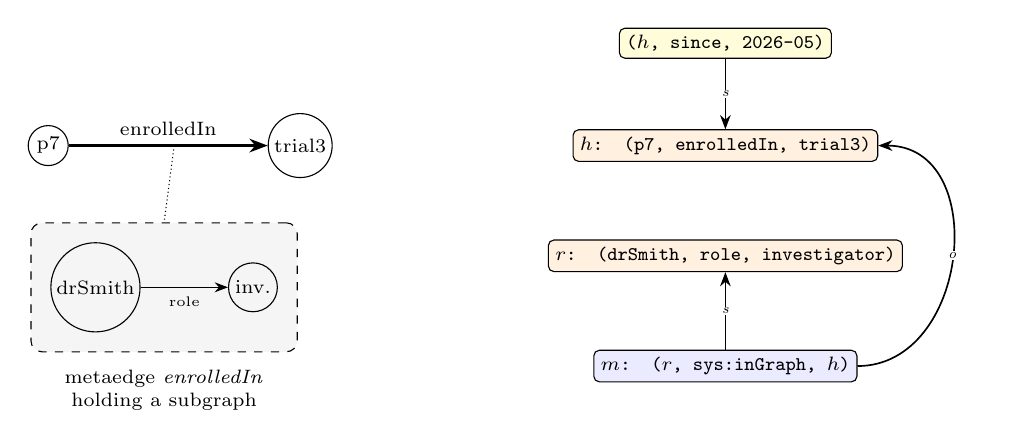
\begin{tikzpicture}[
  st/.style={draw,rounded corners=2pt,fill=#1,inner sep=2.5pt,font=\scriptsize\ttfamily,align=center},
  st/.default=white,
  ref/.style={-{Stealth[length=1.8mm]},semithick},
  lab/.style={font=\tiny\itshape,fill=white,inner sep=.5pt}]
\begin{scope}[shift={(-6.4,0)}]
  \node[circle,draw,inner sep=1.5pt,font=\scriptsize] (p7) at (0,0.9) {p7};
  \node[circle,draw,inner sep=1.5pt,font=\scriptsize] (tr) at (3.2,0.9) {trial3};
  \draw[-{Stealth},thick] (p7) -- node[above,font=\scriptsize] {enrolledIn} (tr);
  \node[circle,draw,inner sep=1.5pt,font=\scriptsize] (ds) at (0.6,-0.9) {drSmith};
  \node[circle,draw,inner sep=1.5pt,font=\scriptsize] (inv) at (2.6,-0.9) {inv.};
  \draw[-{Stealth}] (ds) -- node[below,font=\tiny] {role} (inv);
  \begin{scope}[on background layer]
    \node[draw,dashed,rounded corners,fit=(ds)(inv),inner sep=7pt,fill=gray!8] (box) {};
  \end{scope}
  \draw[densely dotted] ($(p7)!0.5!(tr)$) -- (box.north);
  \node[font=\scriptsize,align=center,below=3pt of box] {metaedge \textit{enrolledIn}\\holding a subgraph};
\end{scope}
\node[st=yellow!15] (a) at (2.2,2.2) {($h$, since, 2026-05)};
\node[st=orange!12] (h) at (2.2,0.9) {$h$: (p7, enrolledIn, trial3)};
\node[st=orange!12] (r) at (2.2,-0.5) {$r$: (drSmith, role, investigator)};
\node[st=blue!8] (m) at (2.2,-1.9) {$m$: ($r$, \sys{inGraph}, $h$)};
\draw[ref] (a) -- node[lab]{s} (h);
\draw[ref] (m) -- node[lab]{s} (r);
\draw[ref] (m.east) to[out=0,in=0,looseness=1.3] node[lab,pos=.5]{o} (h.east);
\end{tikzpicture}
\caption{A metaedge holding a subgraph, and its encoding with the compact
binary form of Remark~\ref{rem:binary}. Retracting $h$ cascades to the
membership $m$ and the annotation, and leaves the contained statement $r$ live:
the container goes, its contents stay (Corollary~\ref{cor:container}).}
\label{fig:metaedge}
\end{figure}

\begin{definition}[Encoding normal form]
A static LBG is in encoding normal form if every row is exactly one of the four
shapes in Definition~\ref{def:enc}. Vertex and edge anchors use their distinct
predicates and a distinct node $n_x$ per atom. Each role has an edge-anchor
subject and an anchor object different from its subject; each edge anchor has
at least one source and target role. There is exactly one role occurrence per
(edge, role kind, endpoint). Memberships have distinct anchor subjects and
objects. Annotations have anchor subjects, non-reserved keys and literal
objects. All referenced anchors exist. A temporal normal form additionally
requires each role's lifetime and valid interval to equal those of its edge anchor.
\end{definition}

\begin{definition}[Decoding]
On encoding normal form, $\dec$ creates one vertex or edge per anchor. Role
objects supply the edge's source and target sets and its anchor object supplies
the edge label. Every membership or annotation row creates its own component
occurrence. In temporal normal form, clocks are read from the corresponding
anchors or component rows. Role clocks need not be stored twice in the decoded model.
\end{definition}

\begin{theorem}[Faithful encoding]\label{thm:faithful}
For every metagraph $M$ with non-reserved annotation keys,
$\dec(\enc(M))\cong M$. Conversely, for every static LBG $G$ in encoding normal
form, $\enc(\dec(G))\cong G$. Thus the static image is exactly that normal
form up to identifier renaming. The same roundtrips preserve all clocks for
temporal normal form.
\end{theorem}

\begin{proof}
The two anchor predicates distinguish atom kinds even when an edge label is
\mg{Vertex}. Decoding assigns each anchor its atom and each role its unique
endpoint in the appropriate set. Each membership and annotation retains its
occurrence identity. This recovers $M$ component by component. Conversely,
normal-form role uniqueness prevents decoding from merging duplicate roles;
node injectivity and the non-self constraints recover valid anchors and incidences.
Every row is reconstructed by exactly one encoding clause. Role-clock equality
makes the temporal reconstruction exact as well.
\end{proof}

Predicate subject-kind declarations enforce some local shape constraints in the
implementation. Role uniqueness, anchor existence, clock equality and non-empty
source and target sets require additional validation; the current engine does
not enforce the complete encoding normal form automatically.

\begin{remark}[Compact binary edges]\label{rem:binary}
For a binary metagraph, replace each edge's anchor and roles by the statement
$h(x)=(h(y),\mathit{lab}(x),h(z))$. Use labels outside the reserved predicate
set; then an edge row has two anchor endpoints, a vertex row retains its
vertex shape, and membership and annotation shapes remain distinct. The compact
decoder reads each such row as one binary edge. This encoding retains the
component clocks and direct endpoint dependencies. Snapshot commutation and
structural closure apply to it, but LR realisability additionally requires an
acyclic edge-dependency graph. Cyclic binary metagraphs are representable as
static compact LBGs, but cannot be inserted from an empty store under LR.

Using $(n_y,\mathit{lab}(x),n_z)$ instead loses vertex-occurrence dependencies
and is outside the vertex-lifetime lifting claim. In the general encoding,
retracting an endpoint may leave its incident edge anchor after role retraction.
A metagraph-level deletion must also remove incident edge anchors and their
dependents; raw statement cascade alone does not preserve general normal form.
\end{remark}

\subsection{The lifting theorem}

\begin{theorem}[Bitemporal Lifting]\label{thm:lifting}
Let $H$ be a well-formed temporal metagraph in the encoding domain of
Definition~\ref{def:enc}. For every transaction time $t$ and
valid instant $v$, the general encoding satisfies
\begin{enumerate}
\item $\dec(\View{t}{v}(\enc(H)))\cong H(t,v)$;
\item $\View{t}{v}(\enc(H))$ is grounded and is in temporal normal form;
\item if every component lifetime is non-empty, the encoded history is realisable
  by transactions obeying LR.
\end{enumerate}
For the compact binary encoding, (1) and (2) hold with its compact normal form;
(3) additionally requires acyclic edge dependencies and non-empty lifetimes. For an ill-formed binary
history encoded compactly, decoding the ground core of its snapshot gives the
largest dependency-closed component subset. This last claim is not made for
the general anchor-and-role encoding.
\end{theorem}

\begin{proof}
For the general encoding, anchors and component rows inherit their clocks;
all roles of an edge share its anchor's clocks. Hence a snapshot retains the
entire encoding of each live component. Well-formedness retains the required
anchors, so the snapshot equals $\enc(H(t,v))$ and Theorem~\ref{thm:faithful}
applies. This also proves closure and normal form.
For (3), at each transaction insert all new anchors first, then their roles,
memberships and annotations; anchors reference no statements. Before retracting
an anchor, retract component rows and roles ending at that transaction, then
the anchors ending there. Lifetime containment guarantees each referent is live
at insertion and no longer-lived referencing row remains at retraction. The non-empty-lifetime assumption ensures that a dependency is alive at its
dependent's addition time. Empty lifetimes have no snapshot effect, but can
violate LR scheduling when their referents have not yet been inserted; they
are therefore excluded from the realisability claim.
This is a model-level schedule, not a claim that every reserved row is writable
through the current public API.

In compact form, each component's references are exactly its dependencies.
The same snapshot argument applies. If dependencies are acyclic, insert new
edge occurrences in referent-first topological order and retract in reverse
order. Lifetime containment alone does not supply such an order for a cycle.
For an ill-formed compact snapshot, the core retains precisely the components
whose transitive dependencies remain, proving maximality by Lemma~\ref{lem:core}.
General edge anchors do not reference their endpoints, so this last argument
fails for the general encoding.
\end{proof}

This theorem transfers snapshots under explicit well-formedness conditions.
It does not establish that arbitrary statement corrections or cascades preserve
metagraph normal form. General n-ary edges require component-level integrity
validation in addition to reference closure.

\subsection{Consequences for metagraph operations}

\begin{corollary}[Unfold and nesting in time]\label{cor:unfold}
For a well-formed $H$, the members of a container $c$ in $H(t,v)$ are the
subjects of the \sys{inGraph} statements with object $h(c)$ in
$\View{t}{v}(\enc(H))$, and the transitive closure of membership at $(t,v)$ is the
answer of a regular path query over $\enc(H)$ evaluated in that view.
\end{corollary}

\begin{corollary}[Containers retract, contents stay]\label{cor:container}
Retracting the anchor $h(c)$ of a container retracts every membership into $c$,
every annotation on $c$ and every statement resting on those, and retracts a
member anchor only if that anchor transitively references $h(c)$. This is a
statement-level cascade claim; preserving general metagraph normal form can
require further edge removals.
\end{corollary}

\begin{proof}
By Theorem~\ref{thm:cascade}, the cascade is $\dep_X h(c)$. A membership into $c$
has $h(c)$ as its object and so lies in it. A member's anchor lies in it only if
it reaches $h(c)$ through references. The membership row references both anchors;
it creates no outgoing reference from the member anchor to the container.
\end{proof}

\begin{corollary}[Fold is a non-destructive write]\label{cor:fold}
Folding a set $F$ of atoms into a container $c$ at transaction $t$ inserts one
membership per atom of $F$, with $c\notin F$, live anchors and valid intervals
contained in those of both endpoints. It changes no view $V_{t'}$ with $t'<t$, and for every
$t''\ge t$ before any later change and every $v$ in the intersection of the
intervals involved, unfolding $c$ at $(t'',v)$ returns $F$ together with any
earlier members.
\end{corollary}

\begin{proof}
By Theorem~\ref{thm:stability} and Corollary~\ref{cor:unfold}.
\end{proof}

\begin{proposition}[Size]\label{prop:size}
$|\enc(M)|=|V|+|E|+\sum_{x\in E}\bigl(|\mathit{src}(x)|+|\mathit{tgt}(x)|\bigr)+|\mu|+|\alpha|$,
linear in the size of $M$; with compact binary edges, a binary edge costs one
statement.
\end{proposition}

For an admissible correction of a compact container edge, internal memberships
retained in $R$ follow its new identifier, while member anchors retain their
identifiers unless they are themselves in the cascade. A correction of a general
edge anchor must also keep its roles coherent with the patched label and clocks;
Theorem~\ref{thm:supersede} alone does not validate that metagraph-specific operation.

% =====================================================================
\section{Paths Through Time}\label{sec:paths}

Layered graphs make paths across layers natural: a walk can go from a belief to
the fact it rests on, to the source of that fact, through virtual hops from a
statement to its subject or object. On top of the two clocks, a path can also be
required to respect valid time. A walk is \emph{time-respecting} from start time
$\tau_0$ if it can traverse each statement at some instant inside its valid
interval, never going back \cite{kempe2002connectivity,holme2012temporal}. With
$\tau$ the walk's current time, a hop over interval $[a,b)$ is allowed iff
$b>\tau$, and moves $\tau$ to $\max(\tau,a)$.

\begin{proposition}[Earliest arrival with a hop bound]
Fix a finite product of a graph view at transaction time $t$ and a regular-path
automaton, a start instant $\tau_0$, and a finite hop bound $K$. Waiting is
allowed and traversal takes zero time. Every hop, including a virtual hop,
counts toward $K$; virtual hops preserve the current instant.
Let $B_k(z)$ be the least arrival at product state $z$ by walks of at most $k$
hops, with $+\infty$ for unreachable states. Initialise the start to $\tau_0$
and the other states to $+\infty$. Then
\[
 B_{k+1}(z)=\min\left(B_k(z),\min_{w\xrightarrow{[a,b)}z,\,B_k(w)<b}
              \max(B_k(w),a)\right)
\]
(with the analogous time-preserving update for virtual hops) returns the earliest
arrival at every accepting end within $K$ hops. It may be implemented by hop
layers, expanding only strict improvements relative to completed earlier layers;
updates in a new layer must not overwrite the saved labels of the layer being expanded.
\end{proposition}

\begin{proof}
Induct on $k$. A walk of at most $k+1$ hops either already has at most $k$, or
has a last hop appended to a walk of at most $k$. The hop rule is monotone:
a feasible hop at a later instant is feasible at an earlier one and ends no
later. Therefore the best prefix label suffices in the recurrence. For pruning,
a label no better than one from a completed earlier layer is dominated in both
time and hop usage; that earlier label has already propagated its feasible
extensions. A later layer's improvement cannot retroactively dominate a prefix
with more remaining hop budget, so saved current-frontier labels are expanded.
Taking the minimum over accepting automaton states proves the end-arrival claim.
\end{proof}

Keeping only earliest arrival in an arbitrary priority-by-time search is
insufficient under a hop bound: a later arrival using fewer hops may reach an
end that an earlier arrival cannot. The repository's timed reachability search
uses saved hop frontiers, matching the required scheduling discipline. Existing
property tests compare it with brute-force bounded walks. The hop rule follows
standard temporal path semantics \cite{wu2014path}; the explicit bound and
product-state scheduling are part of this proposition. Snapshot lifting alone
does not prove journey equivalence for an arbitrary general n-ary edge traversal.

% =====================================================================
\section{Realisation and Conformance}\label{sec:impl}

\subsection{Tiramemsu}

The model is implemented in Tiramemsu, an embedded graph database written in Rust
over SQLite, queried with SPARQL and Cypher over one store. A statement is one
row $(\mathit{eid},s,p,o,\tadd,\tret,v_{\mathrm{from}},v_{\mathrm{to}},\mathit{ret\_kind})$.
Every identifier is a 64-bit integer with a 4-bit type tag in the low bits, so
statements, nodes, transactions and small literals share one column type and stay
compact as SQLite varints. Permutation indexes are split into partial indexes over
live rows, which serve the current view, and history indexes ordered by
$\tadd$ descending, which support as-of scans with addition-time bounds and residual lifetime
filters. Triggers reject deletion, replacement, and immutable-content updates,
and allow a single retraction. Format 3 adds date guards: statement addition
and retraction use the latest transaction record above the committed watermark.
Raw SQL writers must follow the transaction protocol; deliberate schema or
metadata tampering is outside these guards.
Named graphs, including graphs named by statements, are membership rows in the same
table; a graph costs one row and its index entries per member, and selecting a
graph is a seek on the predicate--object index.

Several results of this paper are checked by property-based tests over random
operation sequences and random layered graphs with reference cycles and
memberships: replay equivalence (Theorem~\ref{thm:stability}); equality of the
read-only dependents, the dry-run cascade and the reverse path query
(Theorem~\ref{thm:cascade}); round-tripping of fact bundles; and time-respecting
search against enumeration (Section~\ref{sec:paths}).

\subsection{Conformance repairs}

Earlier revisions retained four counterexamples against the engine. This
revision implements repairs and changes the retained probes to assert that
those cases are prevented. The probes use a fresh temporary database, and
integration regressions run on both the full SQLite host and the minimal host.

\begin{enumerate}
\item \textbf{Retracted and missing endpoints.} Ordinary assertions and creates
  now require statement-valued subjects and objects to name live rows. Checks
  run before writing and again after cardinality replacement, which can retract
  a proposed endpoint through its cascade. Unknown and retracted targets are
  rejected. The engine's reserved \texttt{sys:supersedes} lineage may name
  allocated historical occurrences; it cannot name missing ones. There is no
  general user-defined lineage registry in this implementation.
\item \textbf{Dropped membership layers.} Before allocating copies, correction
  selects foreign memberships and propagates exclusion through their structural
  dependents inside the cascade. Only retained rows receive fresh identifiers.
  A dropped root is rejected. Layers of dropped memberships therefore remain
  historical rather than pointing to copies that were never inserted.
\item \textbf{Patched and external references.} A root object naming a retained
  cascade member is substituted to its fresh copy. Direct self-reference and
  patched references to dropped rows are rejected. External structural targets
  are checked after schema effects and before replay. This can preserve a
  complete cyclic retained graph, without promising acyclic correction.
\item \textbf{Backdated SQL writes.} Format 3 adds insertion and retraction date
  triggers. A date must equal the latest transaction record and exceed the
  committed \texttt{meta.last\_t} watermark; retraction cannot precede addition.
  Insert-then-retract within one transaction remains valid. Opening format 1 or
  2 files migrates forward atomically without rewriting historical rows.
\end{enumerate}

The original four probes now report prevention. Additional regressions check
recursive annotation exclusion, patched-reference substitution, invalid-patch
rollback, cardinality side effects and migration. Existing cycles and invalid
references in old files are not rewritten or repaired during migration: they
still require integrity validation or sanitation before applying complete-carrier
results. Raw SQL bypasses other engine checks; the date guards do not establish
full referential integrity for arbitrary SQL writes. They assume engine metadata
and triggers have not been deliberately modified. The result is evidence for
these repaired contracts, not a universal implementation-conformance proof.

\subsection{Illustrative agent-memory correction workflow}

Consider an assistant storing an employment claim $r$ together with a
confidence layer $c$, a document-evidence layer $d$, and a membership $m$ in a
session container outside the correction cascade. These are distinct statement
occurrences; their transaction clocks record when the assistant committed them,
while the employment claim's valid interval records the claimed employment period.
If $m$ has an annotation $a$, dropping $m$ also requires dropping $a$ under
structural retention. A later document changes the employer named by $r$.
This example is an application policy, not a measured agent-memory experiment.

The application first separates annotations by meaning. Confidence $c$ and
evidence $d$ describe the old employer claim, so copying them unchanged would
misrepresent the replacement. Select them for exclusion along with foreign
membership $m$, and compute the induced structural core of the remaining
cascade. Require that the root survives. The correction theorem applies to this
structurally closed retained set: substitute retained identifiers, patch the
root object, retract the original cascade, and add the predecessor lineage.
Create fresh confidence and evidence rows only after checking the new claim
against the new document. These subsequent assertions obey LR and receive their
own transaction and valid intervals. The original evidence remains available
in historical views; it is not presented as support for the new employer.

This extends the theorem's foreign-membership selection policy to an explicitly
chosen exclusion set $Q$: use
$R=\core_{\Lin,C}(C\setminus Q)$ and require $r\in R$.
The proof uses only structural closure of $R$, so it applies unchanged.
Policy classification and evidence revalidation are application responsibilities.
A grounded replacement can still be factually wrong; this workflow establishes
reference integrity, not factual accuracy or improved retrieval quality.

\subsection{Retained verification results}

The revision artifact uses seed 20261003. Its finite checker examines 2,470
reference graphs with at most four occurrences and two referents per occurrence,
38,946 row subsets, and 618,820 intersection cases. It checks 19,053 minimal
cascades, 1,730 admissible corrections, 200 general metagraph roundtrips,
8,400 bitemporal snapshots, and 1,000 bounded journeys against enumeration.
All checks pass. Four actual-engine probes now verify prevention of the
previously reported conformance gaps. These results test selected finite contracts; they do not measure
throughput, latency, storage overhead, or agent-memory quality.
The retained workflow check also exercises exclusion and revalidation of
object-sensitive annotations. Commands and limits are in
\texttt{paper/artifact/README.md}; hashes and results are in
\texttt{paper/review-v4/}. The same assistant performed the revisions and
post-revision assessment; an external proof review remains desirable.

% =====================================================================
\section{Discussion}\label{sec:discussion}

\paragraph{Occurrences, not facts.} Identity is per occurrence: two statements may
have equal content, and an idempotent assert decides when a new occurrence is
created. This is what lets a fact have two episodes with disjoint valid intervals,
each with its own annotations. RDF~1.2's many-to-many reifiers are more flexible;
an LBG can model them by a reifier node with ordinary statements, losing the
cascade from fact to annotation, which is the point of identity here.

\paragraph{Why valid time is not clamped.} One could force a layer's valid interval
inside its base's on write. We do not, because annotations are often claims
\emph{about} a fact made at another time. Theorem~\ref{thm:effective} gives readers
the clamped semantics on demand. A schema flag that requests clamping for a given
predicate (for example roles of an n-ary edge, whose validity is the edge's) would
make the reader-side core unnecessary for those predicates.

\paragraph{Branching and merging.} The model has one linear transaction axis.
Speculative transactions are evaluated and discarded, as in Datomic, and never
enter the history. Merging the histories of several agents would need identifiers
that are stable across stores; the implementation reserves bits for an origin, but
merge semantics, and how $\core$ behaves under merge, are open.

\paragraph{Complexity.} Given an in-memory adjacency representation, seed
rows of $X$ with a reference outside $X$ and propagate removal along inverse
references within $X$. Each row and reference is visited once, so the core takes
$O(|X|+|D_X|)$ time, where $D_X$ includes outgoing boundary references and
induced edges. A cascade has the same reachability bound on the visited subgraph.
One effective-validity query costs a support traversal and interval intersections;
computing it separately for all rows can repeat shared support. On an acyclic
history, referent-first dynamic programming computes all effective intervals
in linear adjacency time; cycles require strongly connected components first.
These are graph-algorithm bounds, not measured SQL latency or storage bounds.
The present artifact contains correctness checks, not evidence of performance
at $10^4$--$10^7$ rows. Incremental materialisation is future work.

\paragraph{Limitations.} The theorems are about the data model and its operations,
not about query languages. We have not formalised how SPARQL's default graph or
Cypher's dual view of statements interact with $\core$. The conformance findings
have executable repairs, but not every theorem hypothesis has been audited
across every operation. The empirical evidence remains the project's test suite,
not an independent benchmark.

% =====================================================================
\section{Conclusion}

Recursive references between statement occurrences make temporal integrity an
operational concern. On a complete history, the standard down-set interior
characterises closed views and minimal cascades. Lifetime containment and
effective validity describe when snapshots retain their dependencies; admissible
correction preserves structural closure while recording the predecessor.
An explicitly typed metagraph encoding transfers well-formed snapshots, with
additional conditions for compact insertion and general edge operations.
The four identified implementation gaps have executable repairs. Retained checks
exercise their boundary conditions without certifying every operation. These results
support an integrity calculus for agent-memory storage, without asserting
semantic truth preservation or unmeasured performance.

\paragraph{Availability.} Tiramemsu is available at
\url{https://github.com/Volland/tiramemsu} under MIT and Apache-2.0 licences.
This preprint is CC BY 4.0. Revision~4 includes the retained artifact in
\texttt{paper/artifact/}, with commands, fixed model-check seed, engine probes,
source hashes and tool versions. The inspected implementation base is commit
\texttt{fa7880b192a4db3256f0}\allowbreak\texttt{f8cfe2394825a0741e4c}; the workspace also contains
uncommitted work, so the artifact manifest hashes the relevant source files.
A permanent archived release DOI is still needed before submission.

\paragraph{Evidence limits.} The artifact checks finite cases and selected
engine scenarios; it is not a machine-checked proof, an independent performance
benchmark or an agent-memory quality evaluation. The four reported engine gaps
have been repaired and regression-tested; this does not establish universal
conformance or sanitize previously stored invalid histories.

\bibliographystyle{plainnat}
\bibliography{references}

\end{document}
